\documentclass[tikz,border=2mm]{standalone}
\usetikzlibrary{positioning,arrows.meta}

\begin{document}
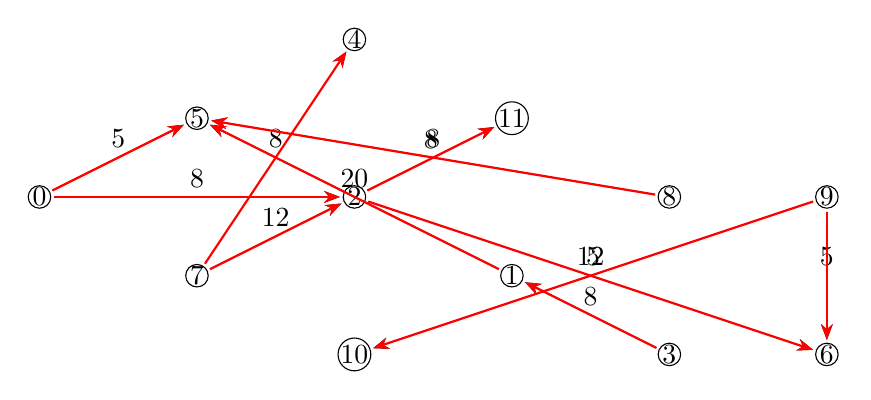
\begin{tikzpicture}[
    node distance=2cm,
    vertex/.style={circle, draw, fill=white, inner sep=0pt, minimum size=2mm},
    edge/.style={draw, -{Stealth[length=2mm]}, shorten >=1pt, shorten <=1pt}
]

% Define vertices
\node[vertex] (0) at (0,0) {0};
\node[vertex] (5) at (2,1) {5};
\node[vertex] (2) at (4,0) {2};
\node[vertex] (11) at (6,1) {11};
\node[vertex] (8) at (8,0) {8};
\node[vertex] (7) at (2,-1) {7};
\node[vertex] (1) at (6,-1) {1};
\node[vertex] (10) at (4,-2) {10};
\node[vertex] (3) at (8,-2) {3};
\node[vertex] (9) at (10,0) {9};
\node[vertex] (6) at (10,-2) {6};
\node[vertex] (4) at (4,2) {4};

% Draw edges
\foreach \u/\v/\w in {0/5/5, 9/10/5, 9/6/5, 0/2/8, 2/11/8, 8/5/8, 7/4/8, 3/1/8, 2/6/12, 7/2/12, 1/5/20} {
    \draw[edge] (\u) -- node[above] {\w} (\v);
}

% Highlight edges in the MST (Kruskal's)

\foreach \u/\v/\w in {0/5/5, 9/10/5, 9/6/5, 0/2/8, 2/11/8, 8/5/8, 7/4/8, 3/1/8, 2/6/12, 7/2/12, 1/5/20} {
    \draw[edge, red, thick] (\u) -- (\v);
}

\end{tikzpicture}
\end{document}
